\chapter{Back-end}

In questo capitolo viene riportata la struttura del Database dell'applicativo.

Il Database utilizzato durante lo sviluppo in locale è stato SQLite3 data la sua portabilità e semplicità di utilizzo, mentre per la versione di produzione è stato utilizzato PostgreSQL, un Database relazionale open source molto diffuso e utilizzato anche da Industry.

Come già affermato in precedenza, uno dei vantaggi di Django è la modularità, difatti è estremamente semplice cambiare il database utilizzato cambiando poche righe di codice, senza dover modificare il codice dell'applicazione.

\section{Migrazioni}
La metodologia con la quale viene aggiornato il database da parte di Django è mediante le \textit{Migrations}, ossia dei file che descrivono i cambiamenti effettuati all'interno del Database. Esse permettono di modificare lo schema del database in modo incrementale e senza dover ricreare il database da zero e senza perdere i dati già presenti.

Nel momento nel quale una migrazione viene creata, Django analizza le differenze tra lo stato attuale rappresentato dai modelli e lo stato precedente salvato nelle migrazioni. Una volta fatto ciò, esso genera un file che contiene del codice python che permette l'interazione con il database.


Uno dei vantaggi del Model View Template presentato nel capitolo \ref{cha:tecnologie_utilizzate} è l'astrazione, difatti per definire il database basta definire i modelli, ovvero le classi che rappresentano le tabelle del database, e Django si occuperà di creare le tabelle e le relazioni tra di esse. Una volta creati i modelli, è possibile creare le migrations, che sono file Python che contengono le istruzioni per modificare lo schema del database mediante un comando apposito. Infine, per poter applicare le modifiche è necessario eseguire un altro comando, che esegue le migrations e modifica lo schema del database.


Ogniqualvolta sia necessario apportare delle modifiche al Database, basterà apportare le modifiche al componente Model, creare le migrazioni ed applicarle. Ovviamente esse permettono in modo estremamente semplice di effettuare il rollback del database ad uno stato precedente nel caso sia necessario annullare le modifiche apportate.

Le migrazioni non sono solo un metodo estremamente efficace per gestire il proprio database, ma permettono anche il tenere traccia dei cambiamenti apportati al database durante la vita dell'applicazione e possono essere facilmente condivise, controllate ed applicate in diversi ambienti di sviluppo da diversi sviluppatori.


In generale, le migrazioni semplificano il processo di gestione del Database fornendo un approccio strutturato ed automatizzato per mantenere il database ed i modelli sincronizzati.

\section{Modelli utilizzati}
In questa sezione vengono riportati i modelli e relazioni tra loro mediante un diagramma semplificato, per evitare di creare confusione al lettore. La notazione scelta è stata l'inserire la cardinalità tra le relazioni, per facilitare la comprensione del diagramma, inoltre la notazione \textbf{[fk id]} indica che la relazione è una foreign key che punta all'id della tabella indicata, mentre la notazione \textbf{[m2m id]} indica che la relazione è una many to many che punta all'id della tabella indicata.

Per migliorare l'esperienza di lettura, sono stati omessi dei dati non necessari, quali i tipi delle variabili ed alcune variabili non necessarie al funzionamento del sistema.

Sono stati anche omessi dei modelli già presenti in Industry che vengono solamente utilizzati per creare un collegamento tra Industry e l'applicativo, come ad esempio il modello \textbf{Company}. 
\begin{figure}[H]
    \begin{center}
        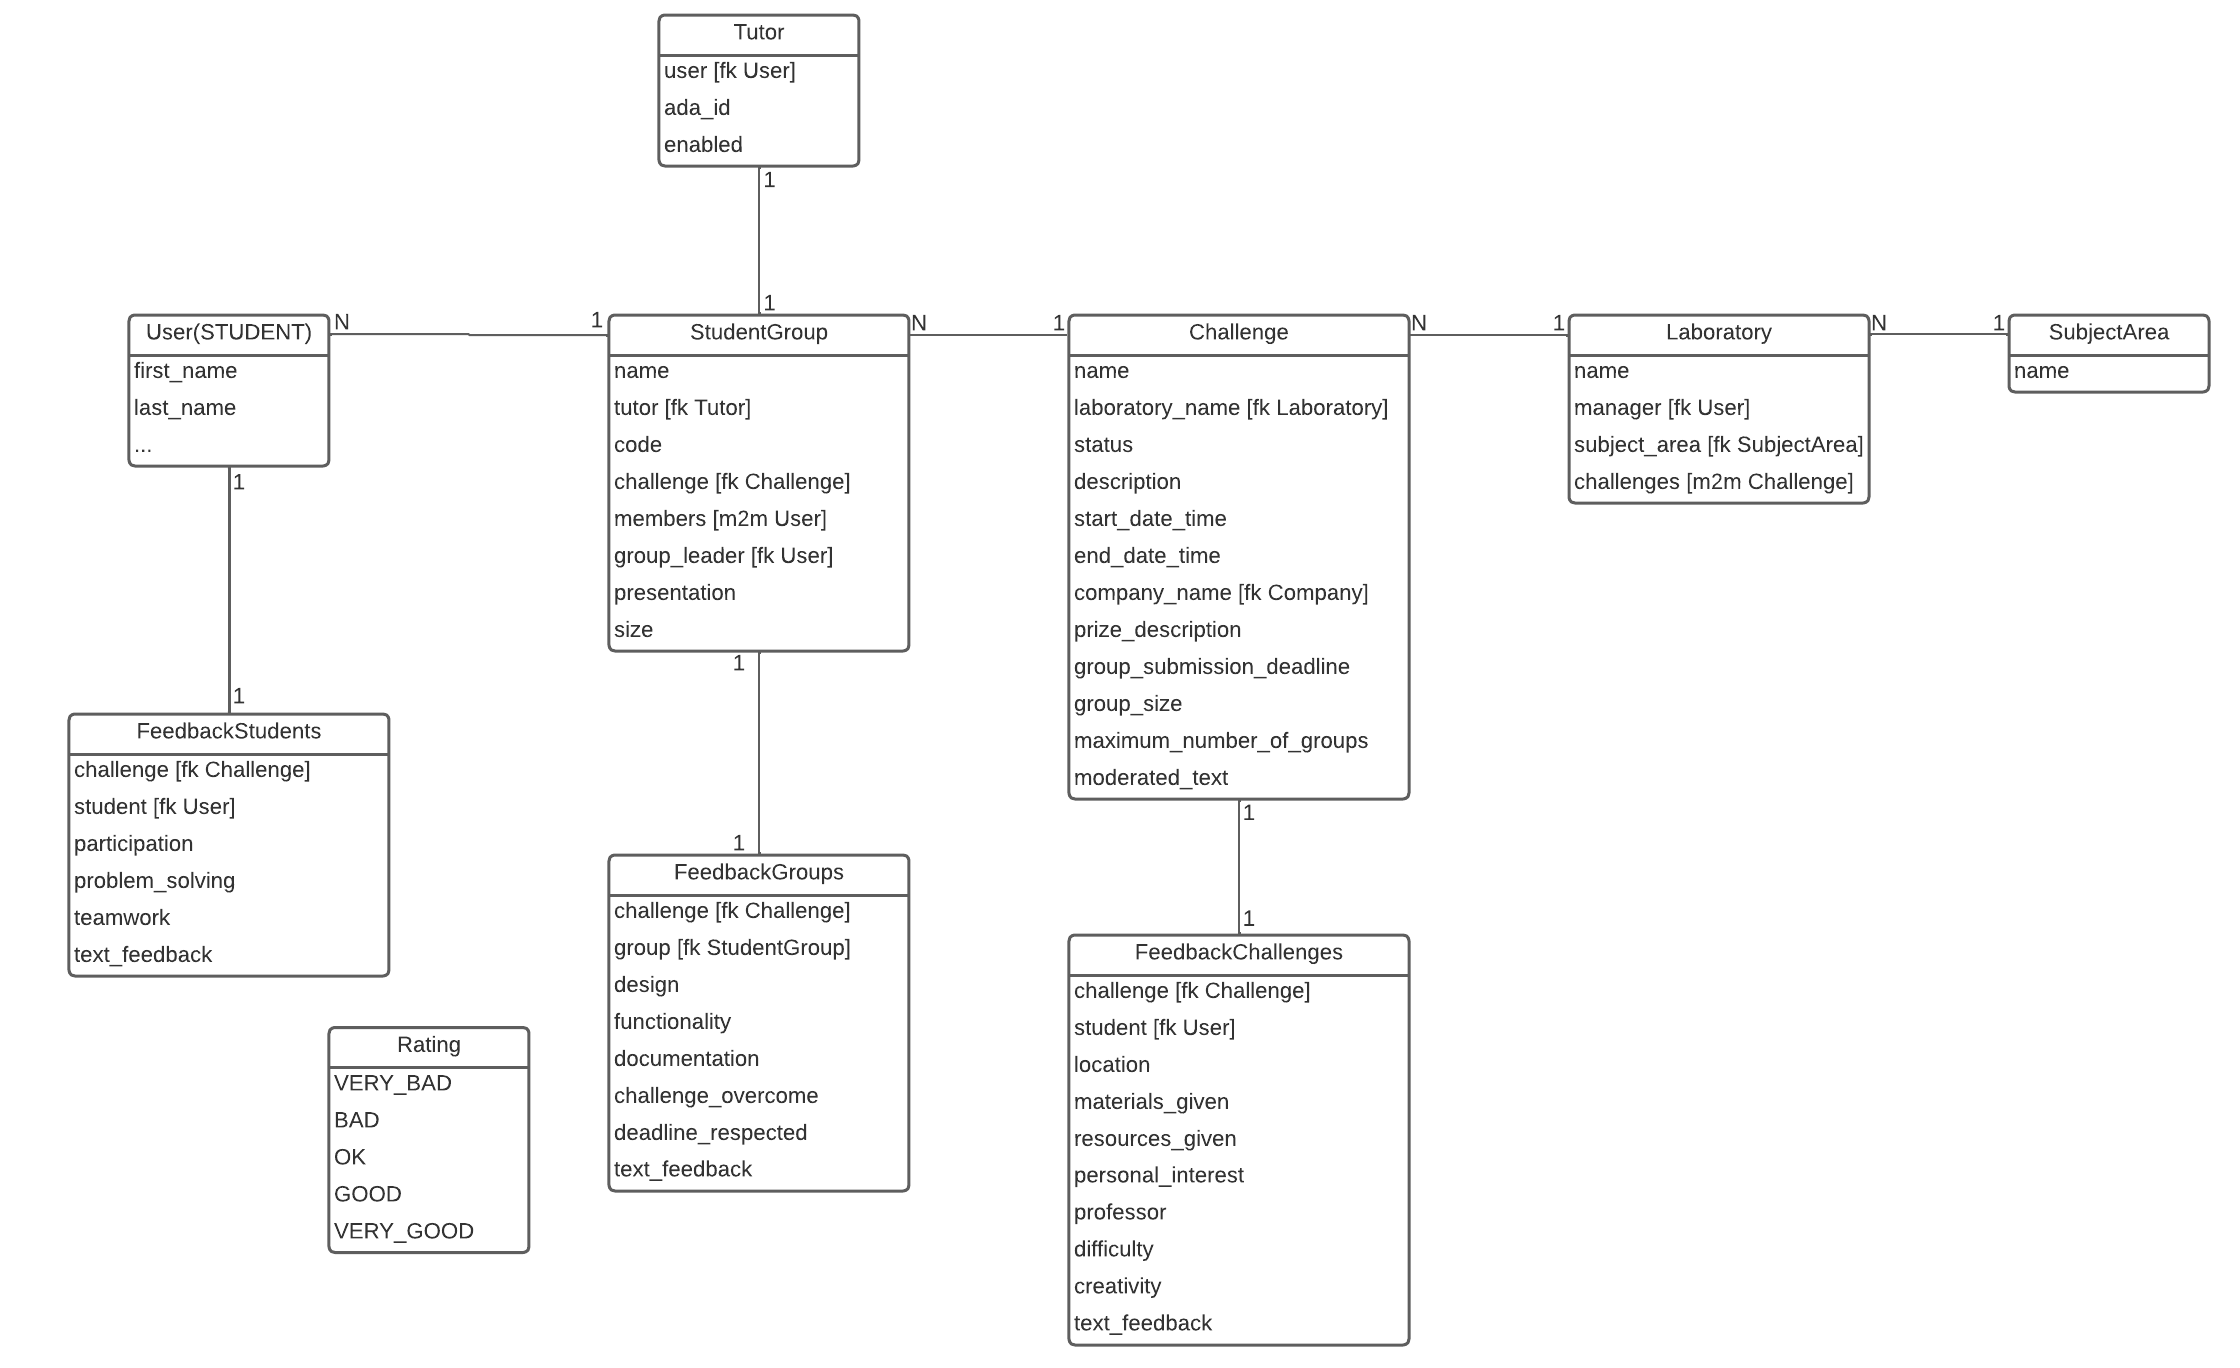
\includegraphics[width=0.95\textwidth]{images/modelli_db.png}
    \end{center}
    \caption{Diagramma semplificato dei modelli utilizzati}
    \label{fig:modelli_db}
\end{figure}

Viene presentata una descrizione dei modelli utilizzati:
\begin{itemize}
    \item User : Modello già presente in Industry, viene riportato per indicare un generico ruolo (in questo caso Student) per poter fornire visivamente il collegamento con FeedbackStudents e StudentGroup. Tale modello detiene, oltre ai dati personali dell'utente, il suo ruolo all'interno del sistema. 
    \item StudentGroup : Modello utilizzato per la rappresentazione di un gruppo creato in occasione della Challenge. Per veicolare la necessità di avere un Tutor per ogni gruppo, è stata inserita una relazione OneToOne con il modello Tutor. Il code è il codice identificativo visibile solamente dal capogruppo ed è necessario per permettere ad esso di invitare altri studenti all'interno di esso.

        Vi è anche l'utilizzo internamente di un \textit{decorator} in \textit{size}, campo il quale rappresenta la dimensione massima del gruppo, per permettere non solo di accedere in maniera veloce alla dimensione dei gruppi riferendosi alla dimensione definita dalla Challenge, ma anche per aumentare la consistenza nel database, in quanto nel caso la dimensione dei gruppi venga cambiata per qualche motivo anche la dimensione massima del gruppo venga aggiornata.
    \item Challenge : Tale modello è composto da i campi definiti nella sezione di definizione di \ref{sec:challenge}. L'unica aggiunta da notare è il campo \textit{moderated text}, che rappresenta il campo testuale compilato dal moderatore in caso di rifiuto della Challenge, come descritto nella sezione adibita alla presentazione del Moderatore \ref{sec:moderatore}.
    \item Laboratory : Questo modello rappresenta il laboratorio nel quale si svolge la Challenge. Esso è necessario per poter accedere ai laboratory gestiti dal moderatore. 
    \item SubjectArea : Questa area rappresenta l'area del laboratorio (Elettronica, Robotica, etc) ed è necessario che sia separata dal laboratorio per modellare l'eventualità nella quale il dipartimento costruisca un ulteriore laboratorio per l'area di interesse definita. 
    \item Rating : Questa è una enum definita per permettere di dare la valutazione a studenti, gruppi e challenge presentata nella sezione \ref{sec:valutazioni}. Ho scelto di dividerlo in 5 valori separati per richiamare il funzionamento del sistema a stelle utilizzato in molti siti web, ad esempio Google Maps.

        Tutti i campi dei modelli Feedback che non siano foreign keys o \textit{text feedback}(il quale rappresenta la descrizione testuale fornita dagli utenti) utilizzano questa enum.
    \item FeedbackStudents, FeedbackGroups e FeedbackChallenges : sono modelli utilizzati per rappresentare le valutazioni fornite da un determinato utente. Essi contengono della ridondanza per questioni di performance, scalabilità e facilità di rappresentazione dei modelli.

\end{itemize}



\clearpage
